\section{Numerical Experiments}\label{sec:chap4 numerical_experiments}
In this section, we demonstrate our pipeline using a small-scale real-world example on Connecticut with five districts $|V|=462,|I|=5$.
The data we use is obtained from the VEST project~\cite{mcdonald2008united} via~\cite{redistrictingdatahub}.
\subsection{Exploratory analysis}\label{sec:connecticut}
We apply the pipeline to redistricting plans of Connecticut, where $|V|=462$ precincts are partitioned into $I=5$ congressional districts.
See Figure \ref{fig:ct_enacted_pop} for the enacted plan in $2022$ and population distribution.
\begin{figure}[!htbp]
    \centering
    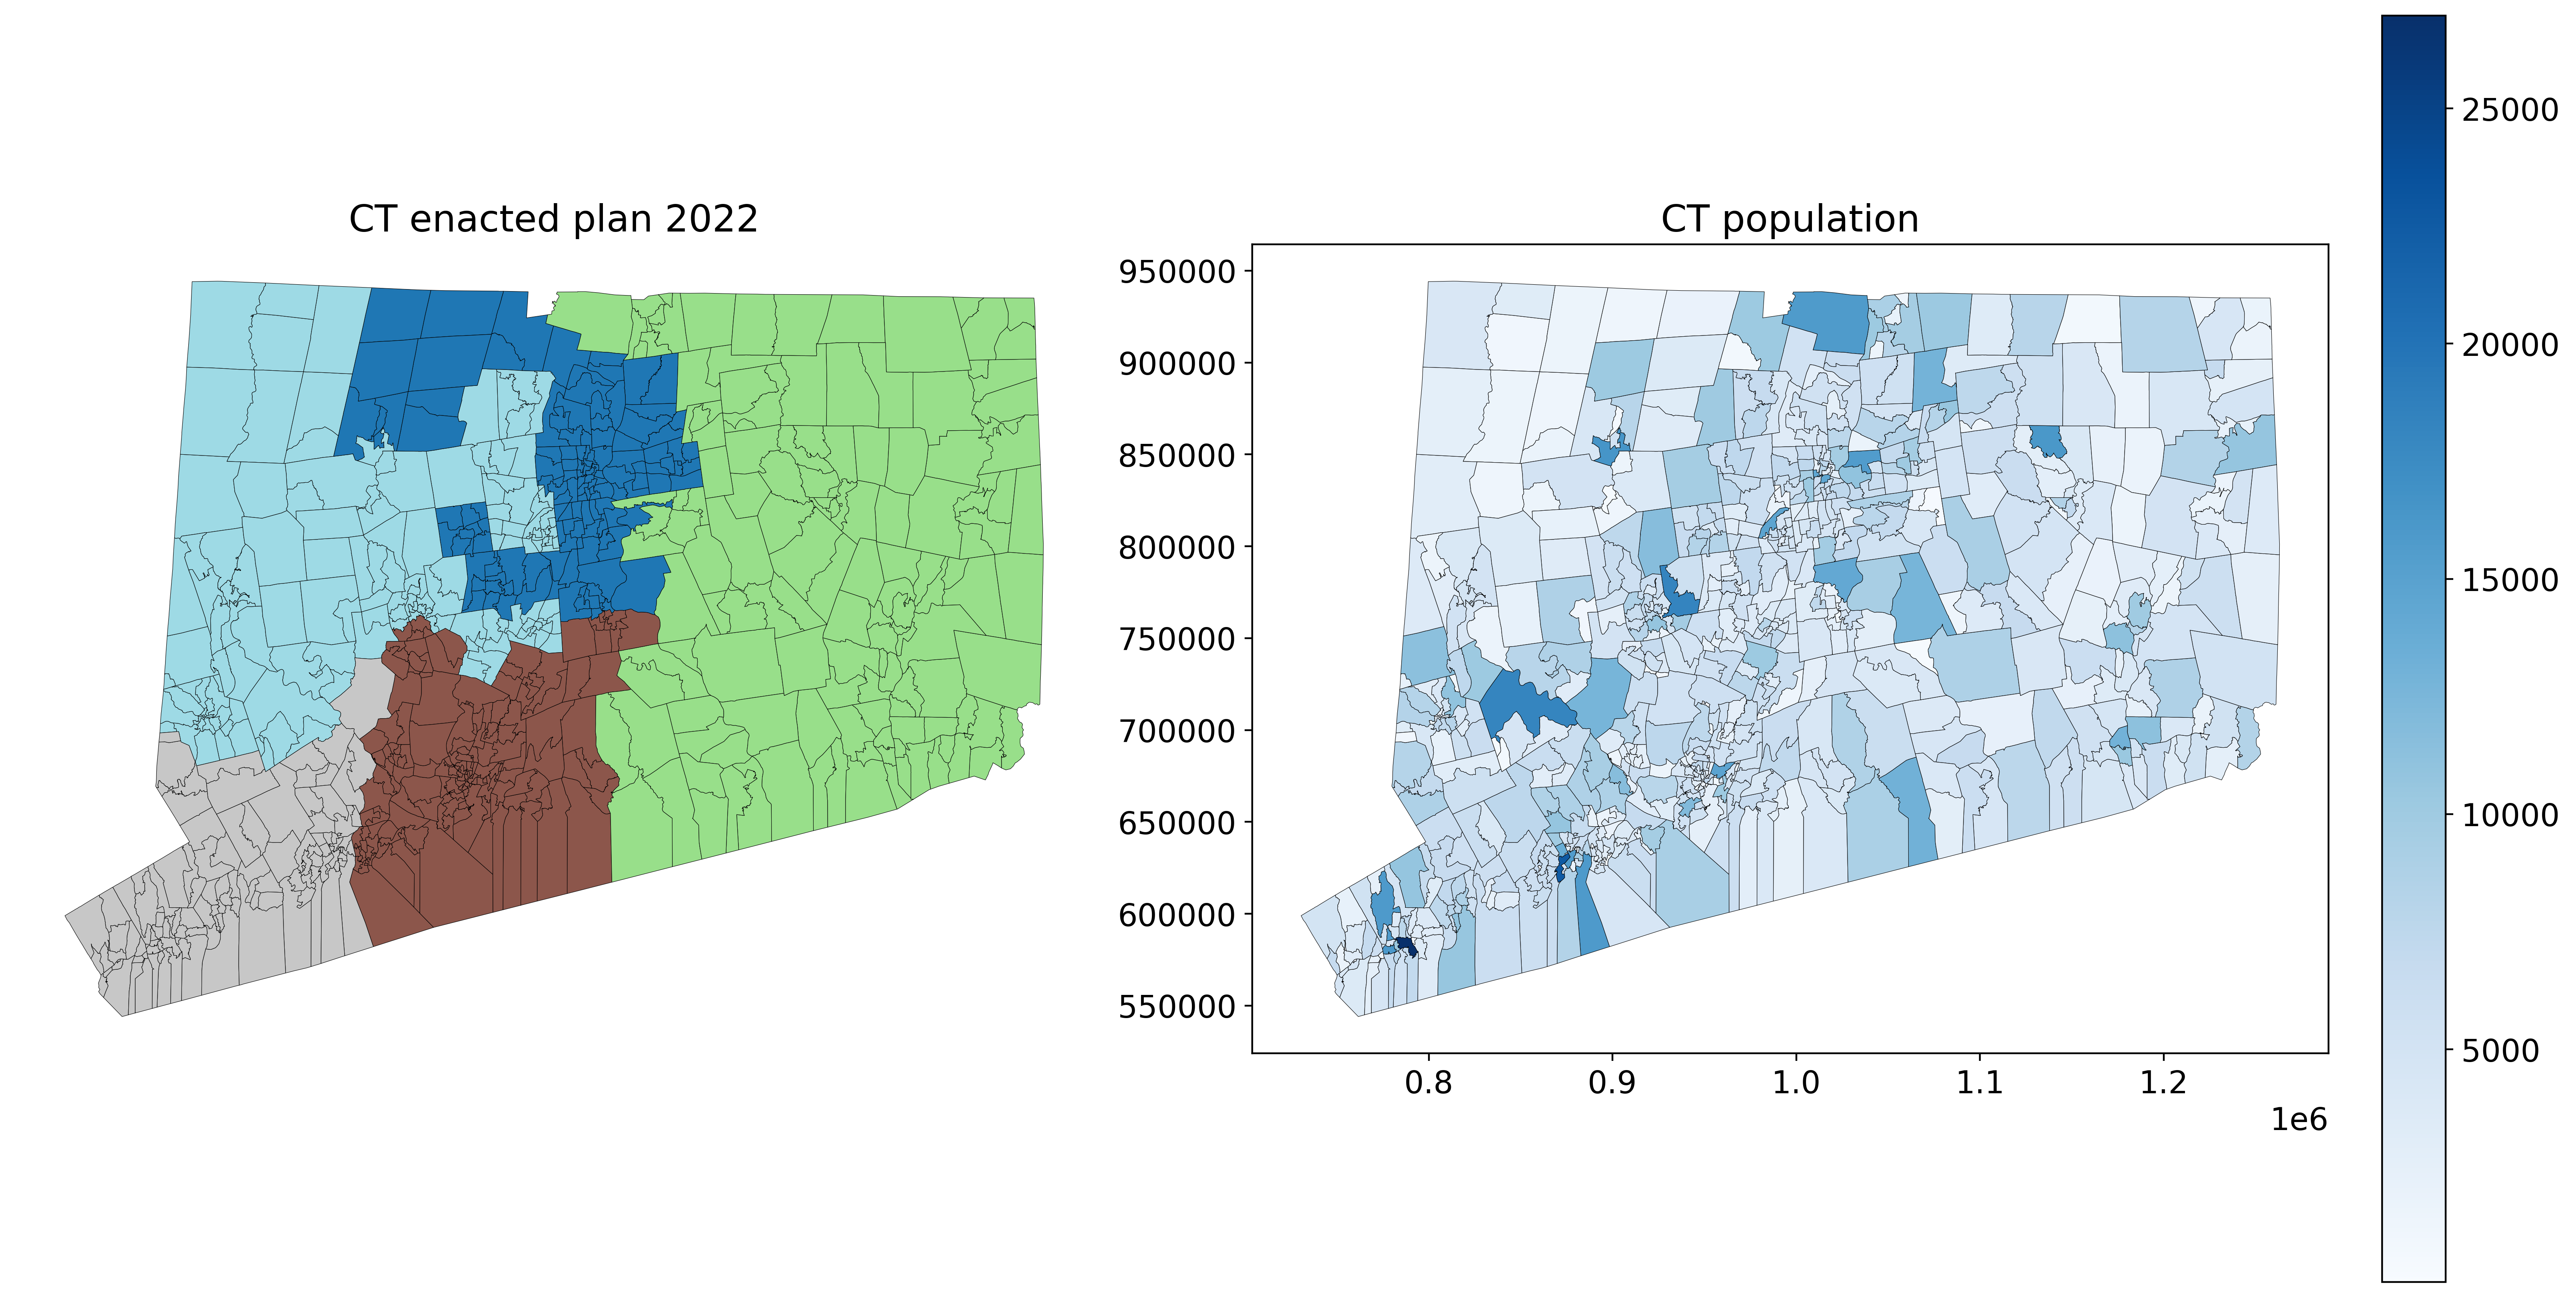
\includegraphics[width=1.0\linewidth]{figures/ct_enacted_pop.png}
    \caption{Population distribution for the enacted Connecticut plan.}
    \label{fig:ct_enacted_pop}
\end{figure}
We work with a $50$K-sample CycleWalk run with $\gamma=0$ (i.e., the tree-count measure).
We notice a clear ``elbow'' in the CT case, where dispersion drops sharply around $K=34$ as shown in Figure \ref{fig:ct_elbow}.
\begin{figure}[!htbp]
    \centering
    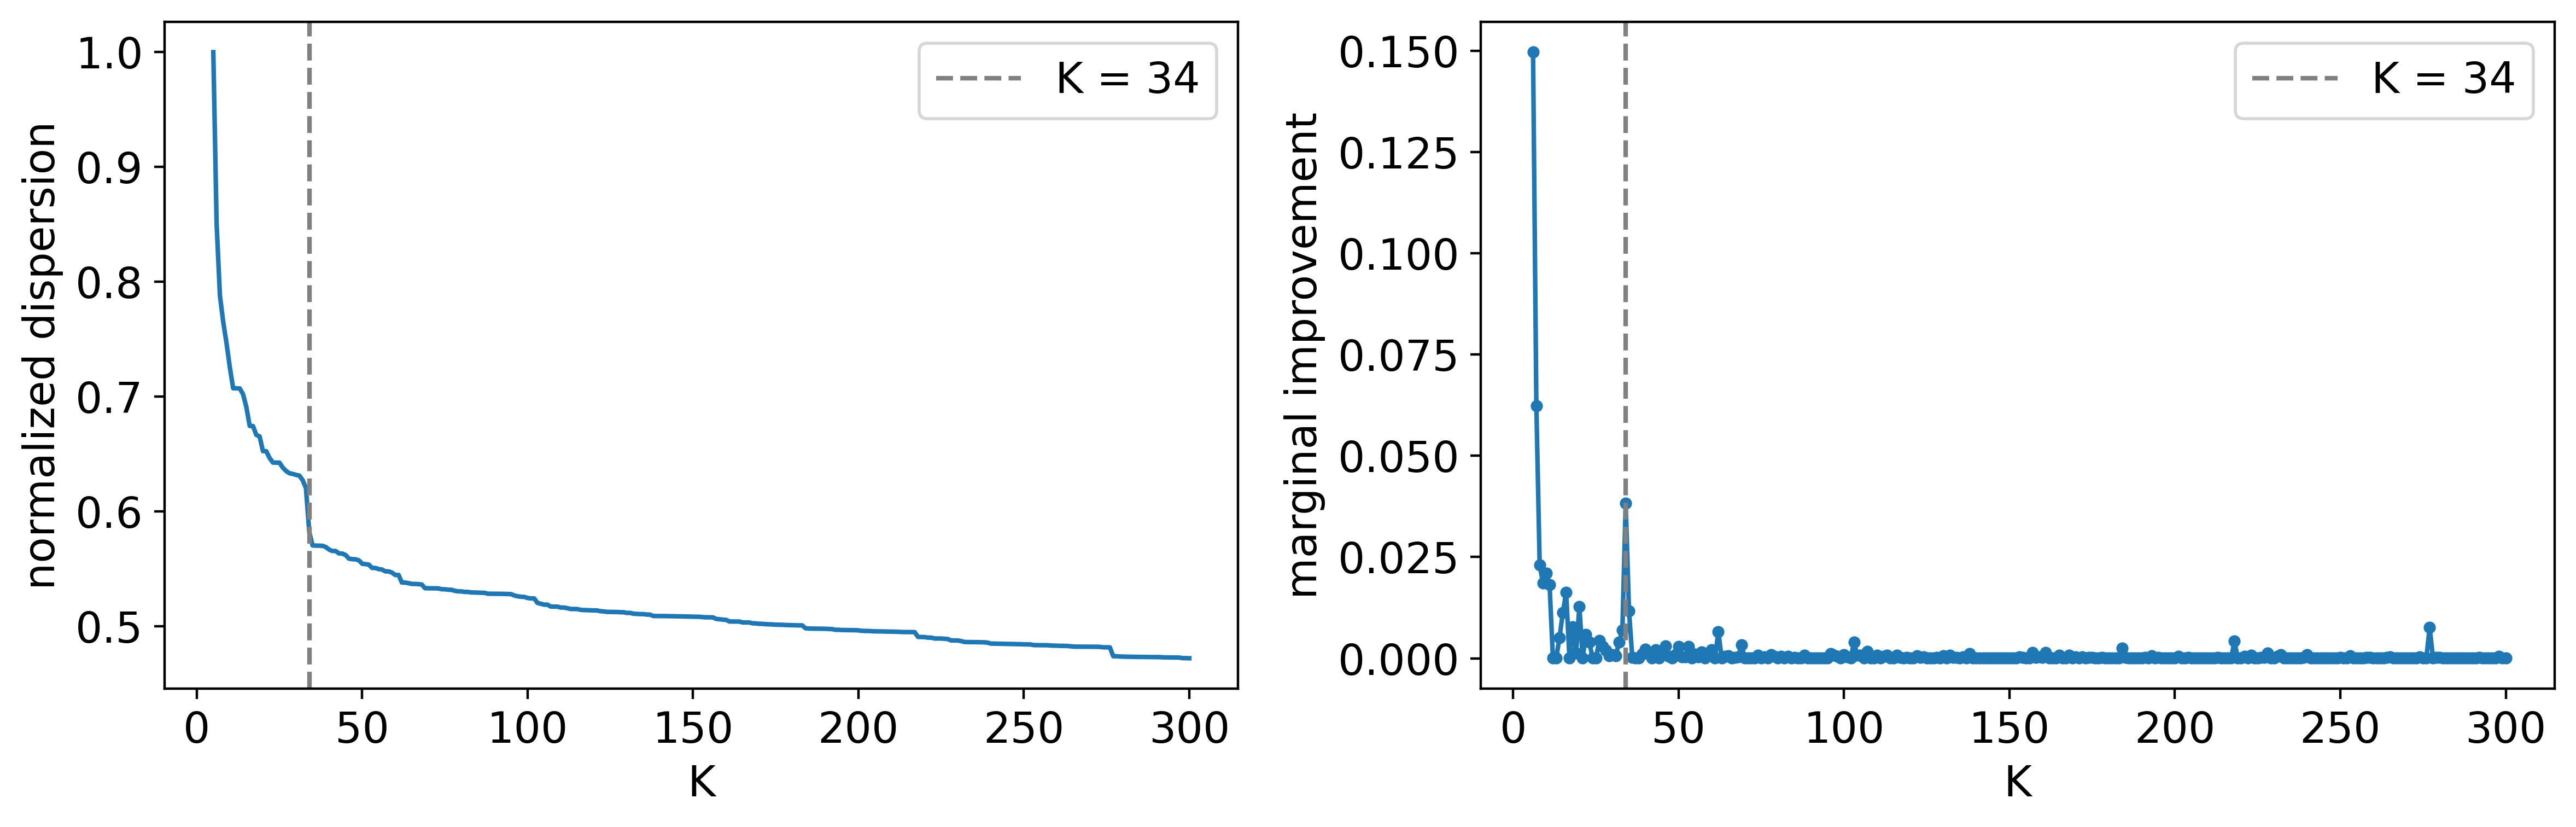
\includegraphics[width=1.0\linewidth]{figures/ct_elbow.png}
    \caption{Elbow plots for CT: left, dispersion metric against number of clusters; right, marginal improvements in the dispersion metric by taking consecutive differences. Dispersion shown is normalized by the first value when $K=5$.}
    \label{fig:ct_elbow}
\end{figure}
Figure \ref{fig:ct_merge_34} shows that the merge of two southwestern clusters corresponds to the sharp drop in dispersion, suggesting an optimal alphabet size of $K=34$.
\begin{figure}[!htbp]
    \centering
    \includegraphics[width=1.0\linewidth]{figures/ct_merge_34.png}
    \caption{Merges of \hccultra around the elbow. Each row shows two child clusters and their merged cluster for a nearby value of $K$. We annotate each merge by the sizes of the clusters involved, as well as the improvement in the dispersion objective. The color on a precinct $p$ indicates the fraction of districts within a cluster that contains $p$.}
    \label{fig:ct_merge_34}
\end{figure}
For the word-level analyses below, we use a slightly finer alphabet with $K=50$ and choose a large beam search width of $L=2000$ to capture the relevant words.
Figure~\ref{fig:ct_top5_word_before_prune} visualizes the five words with the largest observed plan coverage before pruning; several of these high-coverage words are near-duplicates that differ only by small local letter substitutions.
\begin{figure}[!htbp]
    \centering
    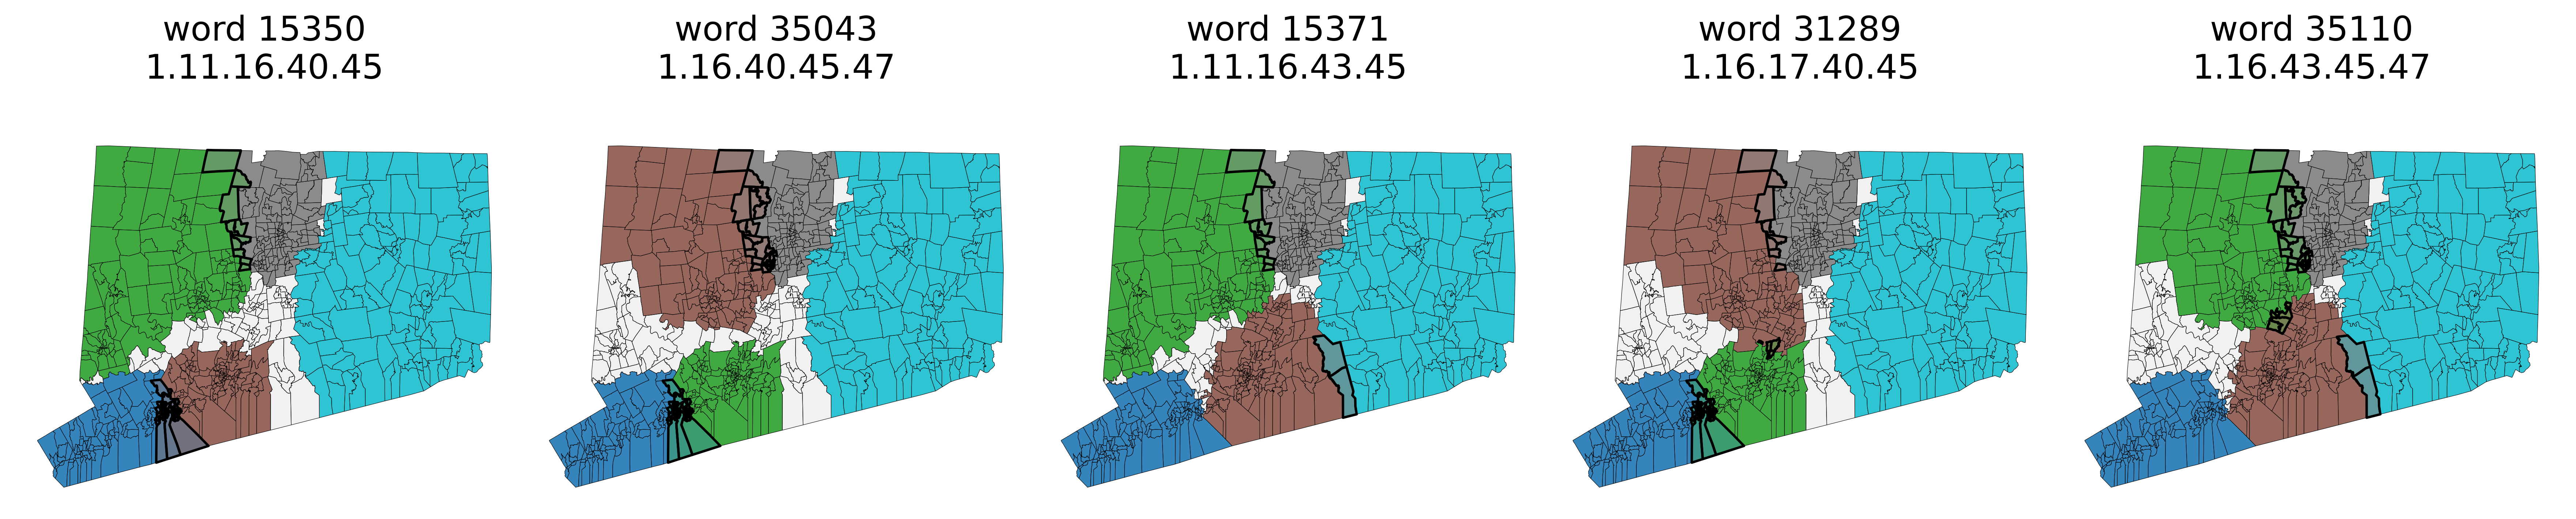
\includegraphics[width=1.0\linewidth]{figures/ct_top5_word_before_prune.png}
    \caption{Top five words (by number of plans covered) before pruning. We visualize words by plotting the letters with different colors. Intersections between letters are highlighted in black lines.}
    \label{fig:ct_top5_word_before_prune}
\end{figure}

To improve interpretability and reduce redundancy while preserving coverage of the observed plans, we construct the pruned set $\mathcal{S}_\eta$ using the two-stage greedy subcover in Algorithm~\ref{alg:eta_greedy_subcover}.
Here we take $\eta=1.0$, which selects $50$ representative words and covers all $49{,}961$ processed plans.
Figure~\ref{fig:ct_top5_word_after_prune} shows that, after pruning, the top words are more diverse and correspond to distinct large-scale plan motifs rather than minor variations within the same mode.
Word $15350$ has the largest coverage and appears in both Figure~\ref{fig:ct_top5_word_before_prune} and Figure~\ref{fig:ct_top5_word_after_prune}; it is selected first in the initial greedy subcover of Algorithm~\ref{alg:eta_greedy_subcover}.
This word is also close to the $2022$ enacted plan.
The southwestern letter (in blue) remains a strong district-level motif after pruning, while the other four districts show more variation across the retained words.

\begin{figure}[!htbp]
    \centering
    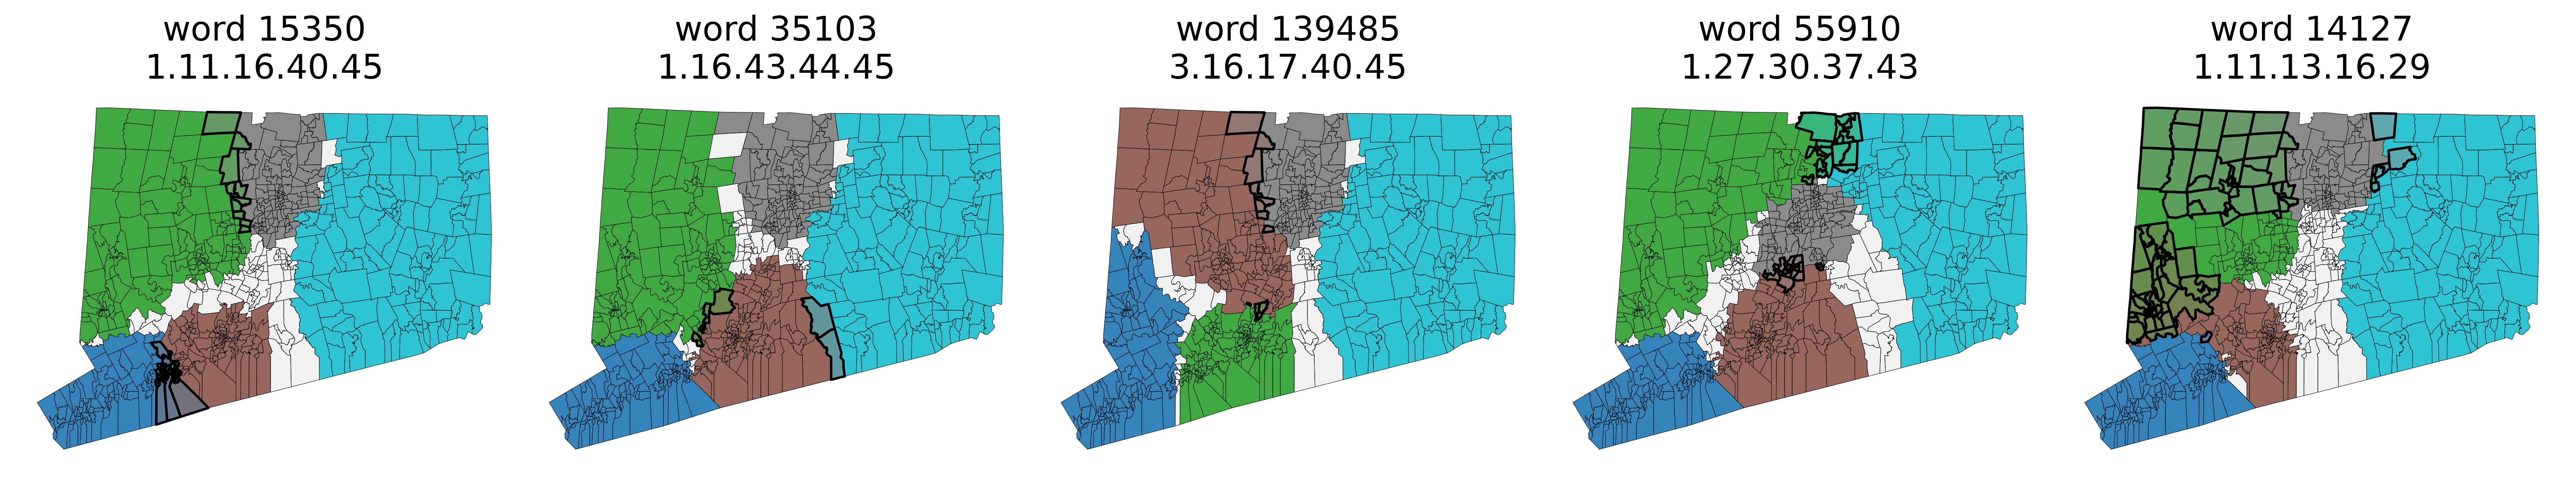
\includegraphics[width=1.0\linewidth]{figures/ct_top5_word_after_prune.png}
    \caption{Similar to Figure \ref{fig:ct_top5_word_before_prune} but for the pruned set $\mathcal{S}_\eta$ produced by the two-stage greedy subcover. Pruning removes near-duplicate strata while maintaining coverage of the sampled ensemble, yielding a more compact and interpretable set of representative words.}
    \label{fig:ct_top5_word_after_prune}
\end{figure}

It is also interesting to see how the enacted plan fits into our strata, even though it follows a quite different measure.
In practice, redistricting plans are typically proposed by legislators and accepted through a political process.
See Figure \ref{fig:ct_enacted_words} for a visualization of the nearest words to the $2022$ enacted plan.
We compare the three closest words before pruning and in the two-stage pruned set $\mathcal{S}_\eta$.
As expected, the minimum distance between the enacted plan and the representative word set increases after pruning, from about $1.34$M to $1.47$M in the displayed distance.
Nevertheless, the closest word in the pruned word set successfully captures the macroscopic spatial structure of the plan.
Note that we do not see any highly specific local boundary geometry even before pruning, e.g. the dark blue district in the north-central region of the enacted plan.
These localized features are intentionally smoothed out during the hierarchical clustering phase, which abstracts districts into representative letters.
\begin{figure}[!htbp]
    \centering
    \includegraphics[width=1.0\linewidth]{figures/ct_enacted_words.png}
    \caption{Closest words to the enacted plan. The first and second rows of the $2\times 3$ word plots show the three closest words after and before pruning, respectively. For each word displayed, we annotate its distance to the enacted plan.}
    \label{fig:ct_enacted_words}
\end{figure}

Next, we compute stationary distributions using multiple choices of temperatures while keeping the range mapping function $\kappa$ fixed.
Typically, we could tune $T$ and $\kappa$ based on empirical observations from stratified sampling.
Since we do not implement stratified sampling in the current paper, we pick a generic $\kappa$ that maps most of the pruned nearest neighbors into the $[0,1]$ range (and zero if a word is not within beam width).
We vary the temperature over $T=0,10,20$ in Figure \ref{fig:ct_stat_flux}.
Specifically, we include the case of $T=0$ (the counting measure) as an example that is $\kappa$ independent.
\begin{figure}[!htbp]
    \centering
    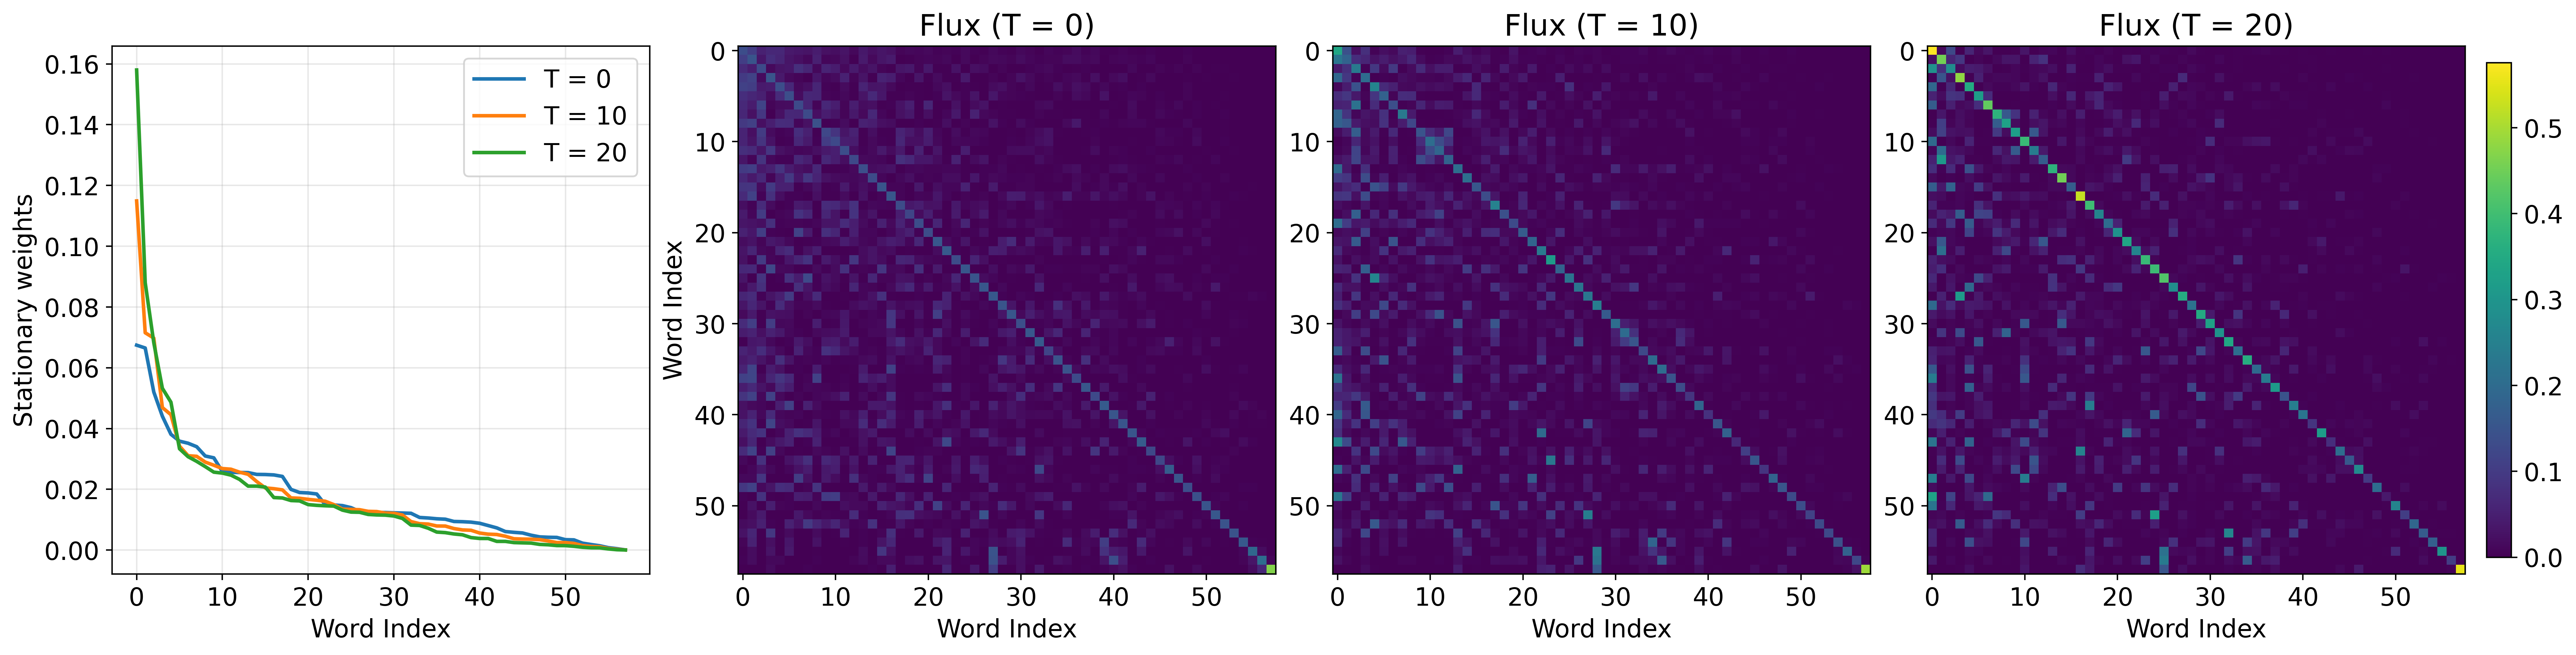
\includegraphics[width=1.0\linewidth]{figures/ct_stat_flux.png}
    \caption{Stratum weights and flux matrices for $T=0,10,20$.}
    \label{fig:ct_stat_flux}
\end{figure}
At the intermediate temperature $T=10$, we see reasonable overlaps across most strata except for the smallest one, which corresponds to an atypical plan.
See Figure \ref{fig:ct_top_bot_words} for more details, where we illustrate the three largest and three smallest strata together with example plans attached to those words.
\begin{figure}[!htbp]
    \centering
    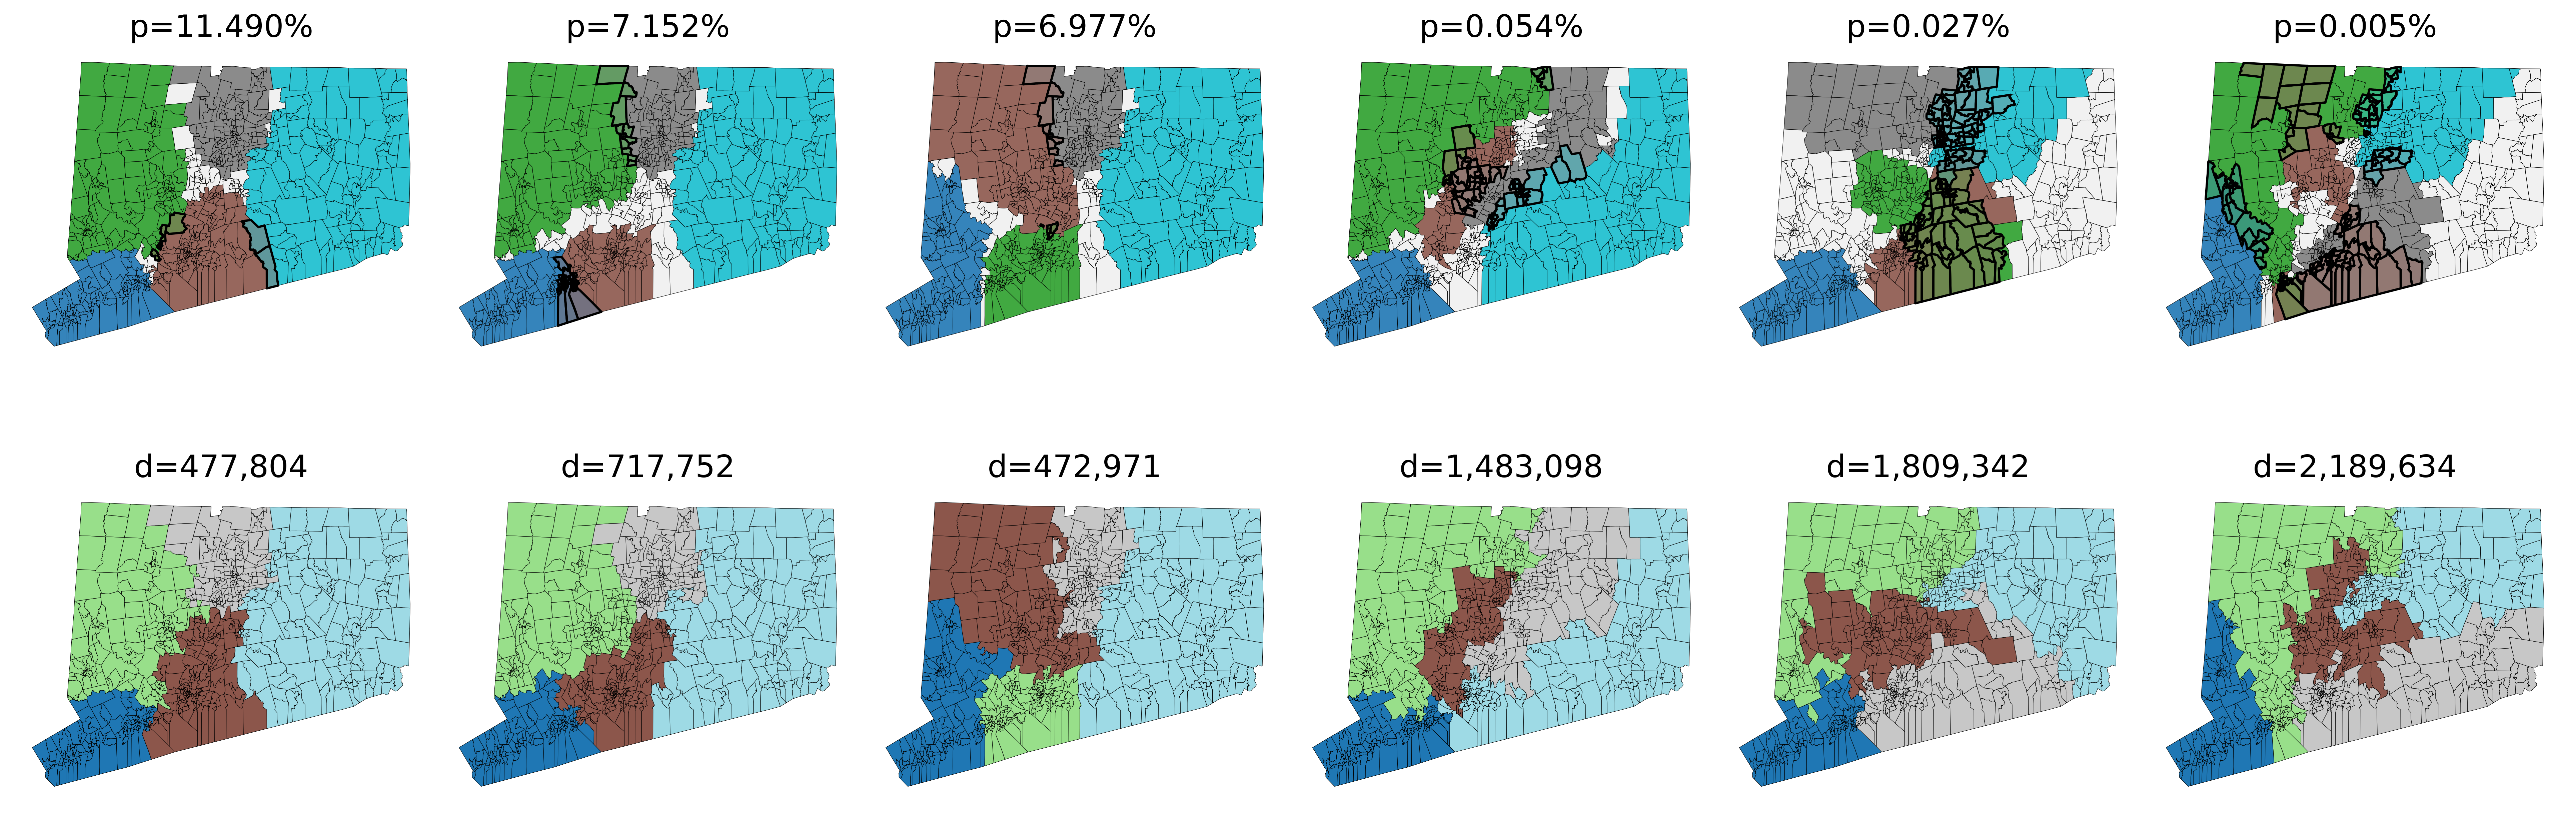
\includegraphics[width=1.0\linewidth]{figures/ct_top_bot_words.png}
    \caption{Top and bottom three words according to the stationary distribution at $T=10$. Words are shown in the first row, and example plans attached to those words are shown in the second row.}
    \label{fig:ct_top_bot_words}
\end{figure}


\subsection{Beyond $\gamma=0$}
In this section, we study how our strata construction generalizes to other $\gamma$.
Same as~\cite{cyclewalk}, we sample from a family of unnormalized probability distributions proportional to $\exp\{-\gamma J_{\mathrm{tree}}(x)-c_\gamma J_{\mathrm{iso}}(x)\}$ parametrized by $(\gamma,c_\gamma)$, where $J_{\mathrm{tree}}$ is the log spanning-forest count and $J_{\mathrm{iso}}$ is the sum of district isoperimetric scores.
We refer to $c_\gamma$ as the iso parameter.
Intuitively, larger iso parameters tilt the target distribution toward smaller isoperimetric scores, i.e., more compact districts.
Meanwhile, increasing $\gamma$ from $0$ to $1$ tilts the distribution more toward uniform partitions, which are less compact.

As a first step, we calibrate the iso parameter to obtain, for each $\gamma$ from $0$ to $1$, an iso parameter that produces samples with isoperimetric ratio comparable to that of $(0,0)$.
We see that the relationship between $\gamma$s and calibrated iso parameters is roughly linear, which is consistent with the observations in~\cite{cyclewalk}.
See Figure~\ref{fig:iso_calibration} for more details.
After calibration, the isoperimetric-score distributions remain comparable across $\gamma$, while the distribution of log spanning-forest counts shifts downward as $\gamma$ increases.
Keeping compactness comparable makes it more reasonable to use strata constructed from one distribution to study another distribution in this family.
\begin{figure}[!htbp]
    \centering
    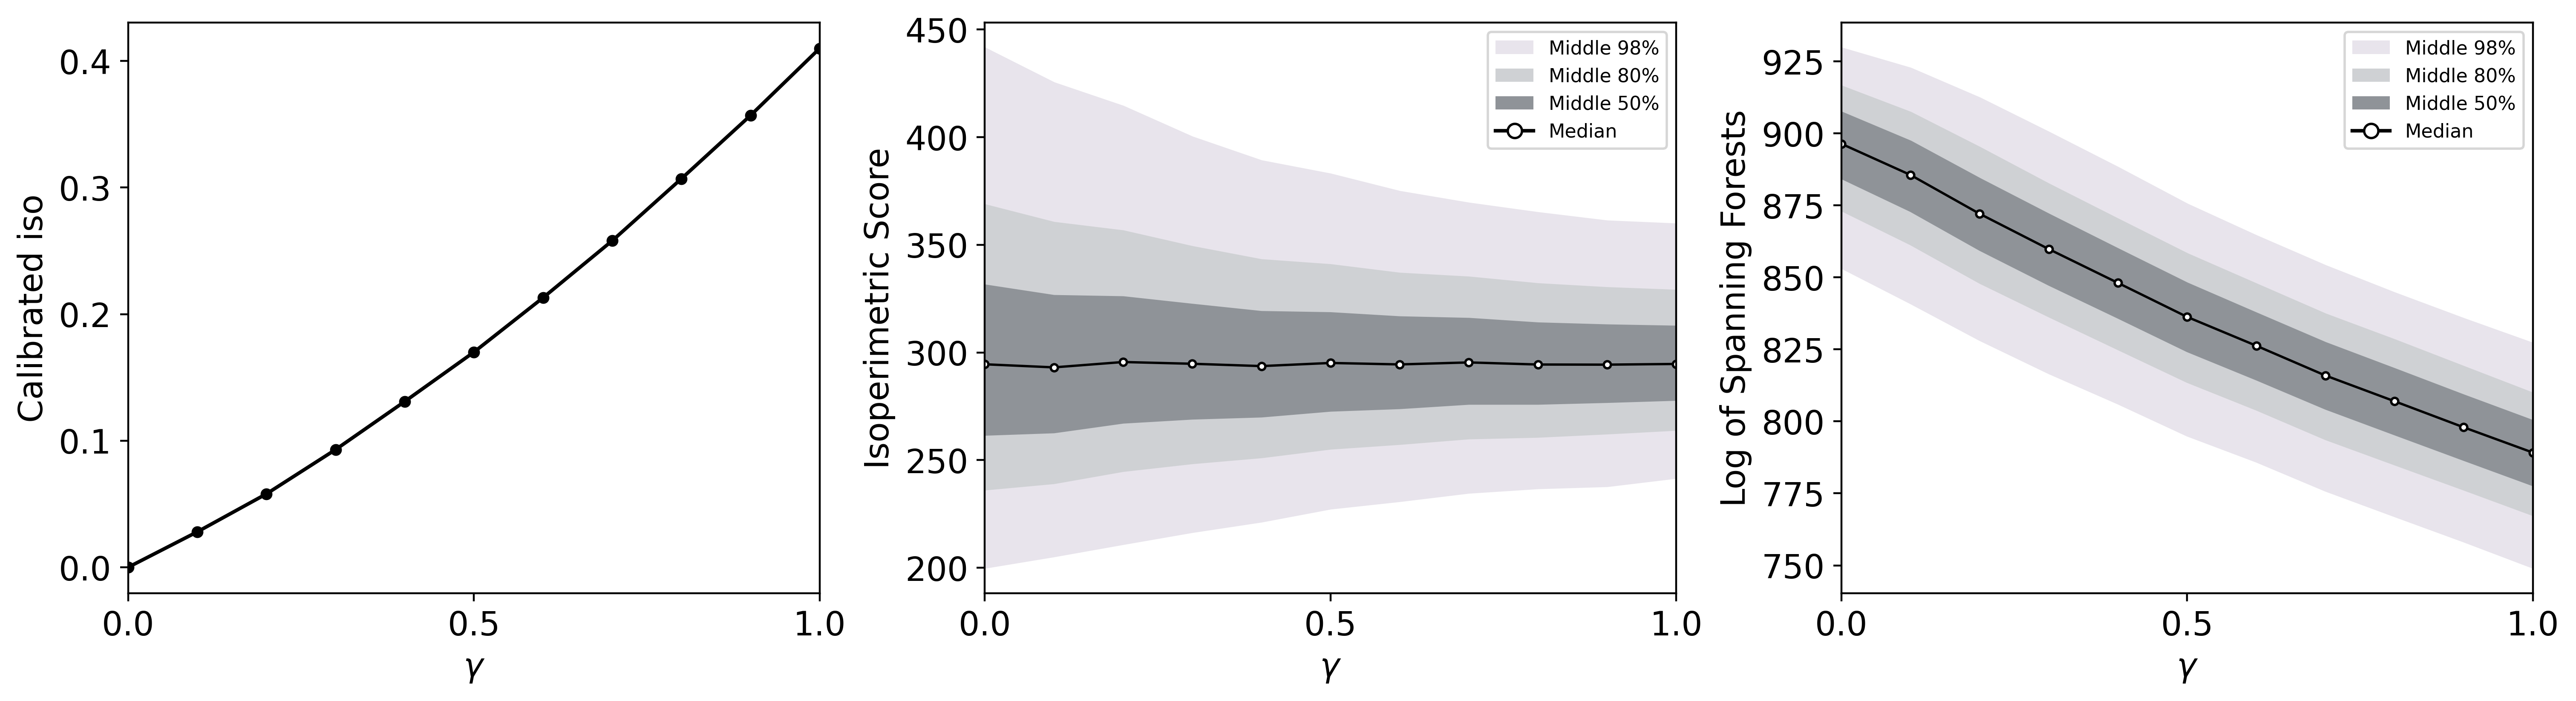
\includegraphics[width=1.0\linewidth]{figures/iso_calibration.png}
    \caption{Calibration of the isoperimetric parameter for target measures indexed by $\gamma$. Left: calibrated iso value for each $\gamma$. Middle: isoperimetric-score distributions, with shaded bands showing the middle $50\%$, $80\%$, and $98\%$ intervals and markers showing medians. Right: distributions of log spanning-forest counts.}
    \label{fig:iso_calibration}
\end{figure}
Figure~\ref{fig:ct_cmds_overlay_seed_A} gives a geometric view of how the sampled district distribution changes as $\gamma$ varies.
To produce this visualization, we compute pairwise weighted $\ell^1$ distances between districts sampled from the three target distributions and project them to two dimensions using classical multidimensional scaling~\cite{torgerson1952multidimensional}.
The three point clouds occupy a common low-dimensional geometry, but their mass shifts as $\gamma$ changes.
This suggests that the alphabet computed with $\gamma=0$, shown as black diamonds in Figure \ref{fig:ct_cmds_overlay_seed_A}, remains informative for other target distributions in this family, while becoming less centered on the target distribution as $\gamma$ moves away from $0$.
\begin{figure}[!htbp]
    \centering
    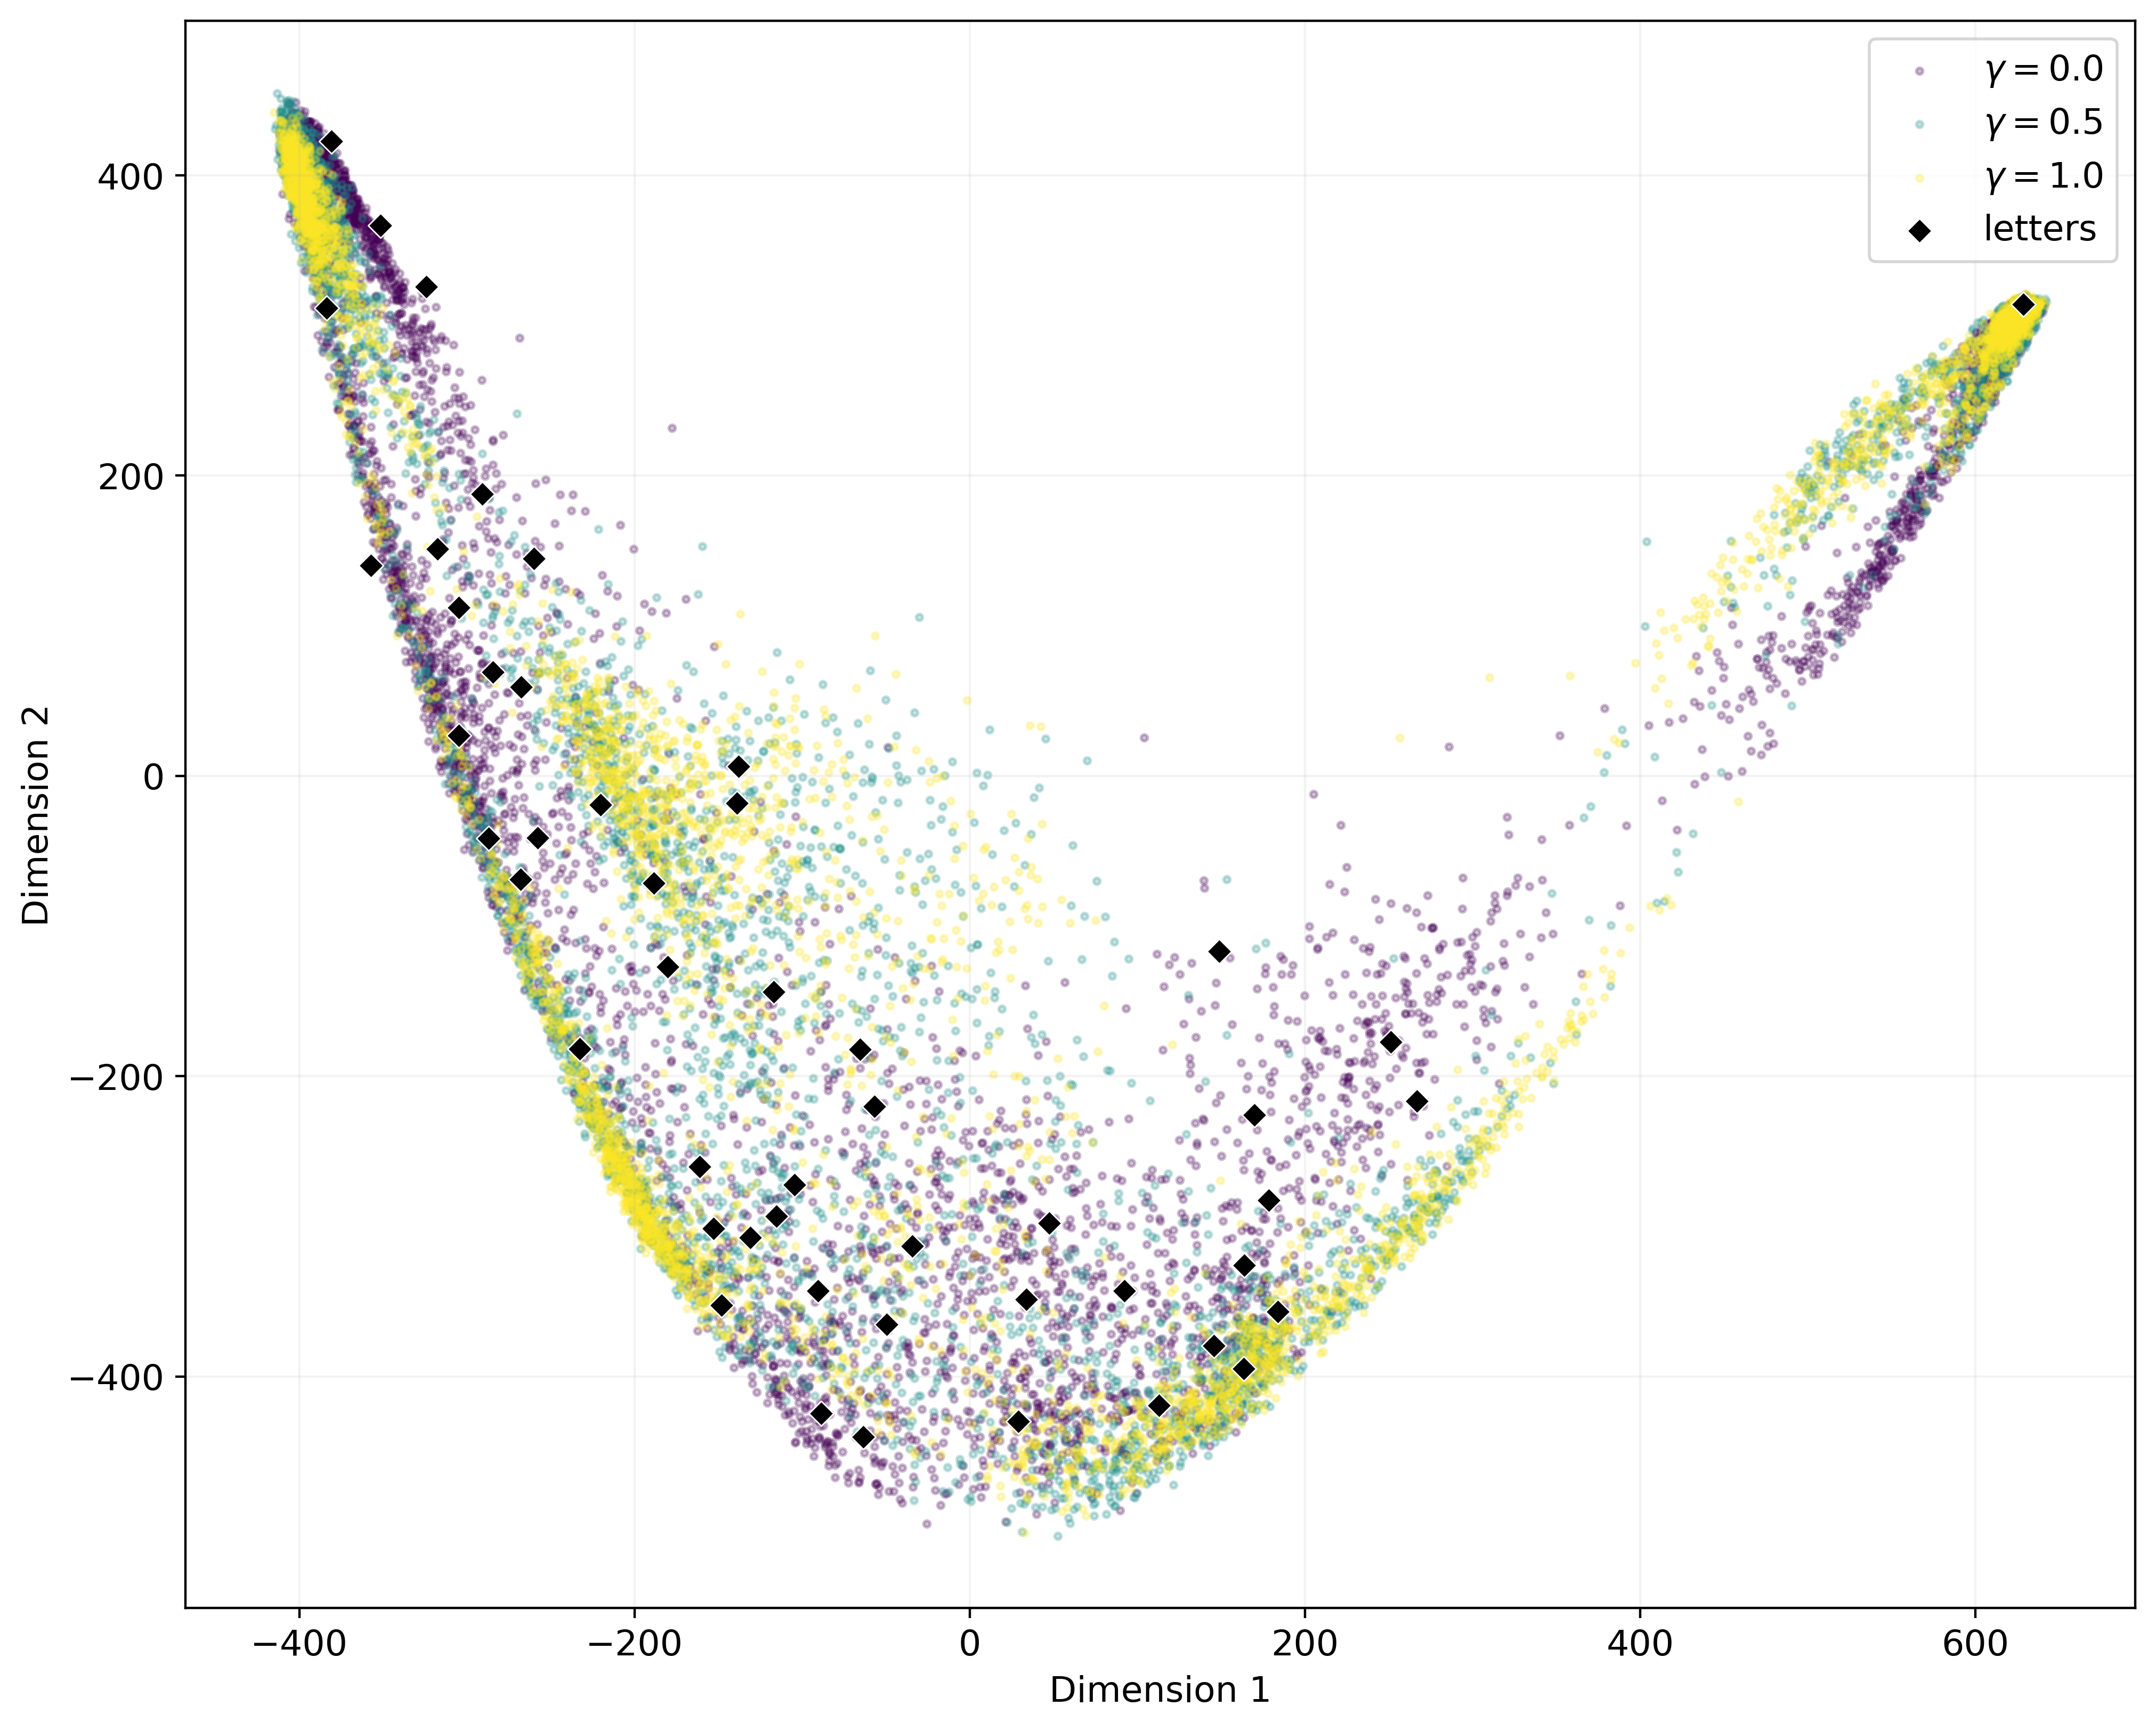
\includegraphics[width=0.92\linewidth]{figures/ct_cmds_overlay_0p0_0p5_1p0_seed_A.png}
    \caption{Classical multidimensional scaling embedding of Connecticut sampled districts for $\gamma\in\{0,0.5,1.0\}$ using seed A. Colors indicate $\gamma$, and black diamonds denote the representative letters learned from the baseline ensemble.}
    \label{fig:ct_cmds_overlay_seed_A}
\end{figure}

In practice, we would like to construct strata using samples from $\gamma=0$, where sampling is relatively cheap, and then use those strata to study other values of $\gamma$.
For this to be reasonable, the resulting words should still have enough overlap under the other target distributions.
As a first sanity check, we fix $\eta=0.70$ and $T=10$ and repeat the computation with two independent runs.
Figure~\ref{fig:ct_gamma_eta_0.70_T_10} shows that the qualitative spectral-gap behavior is consistent across seeds.
The differences between the two flux matrices and stationary distributions grow for larger $\gamma$, which may reflect slower convergence of the underlying chains as the target moves farther from the tree-count measure.
For other combinations of $\eta$ and $T$, we see patterns that are qualitatively similar.
\begin{figure}[!htbp]
    \centering
    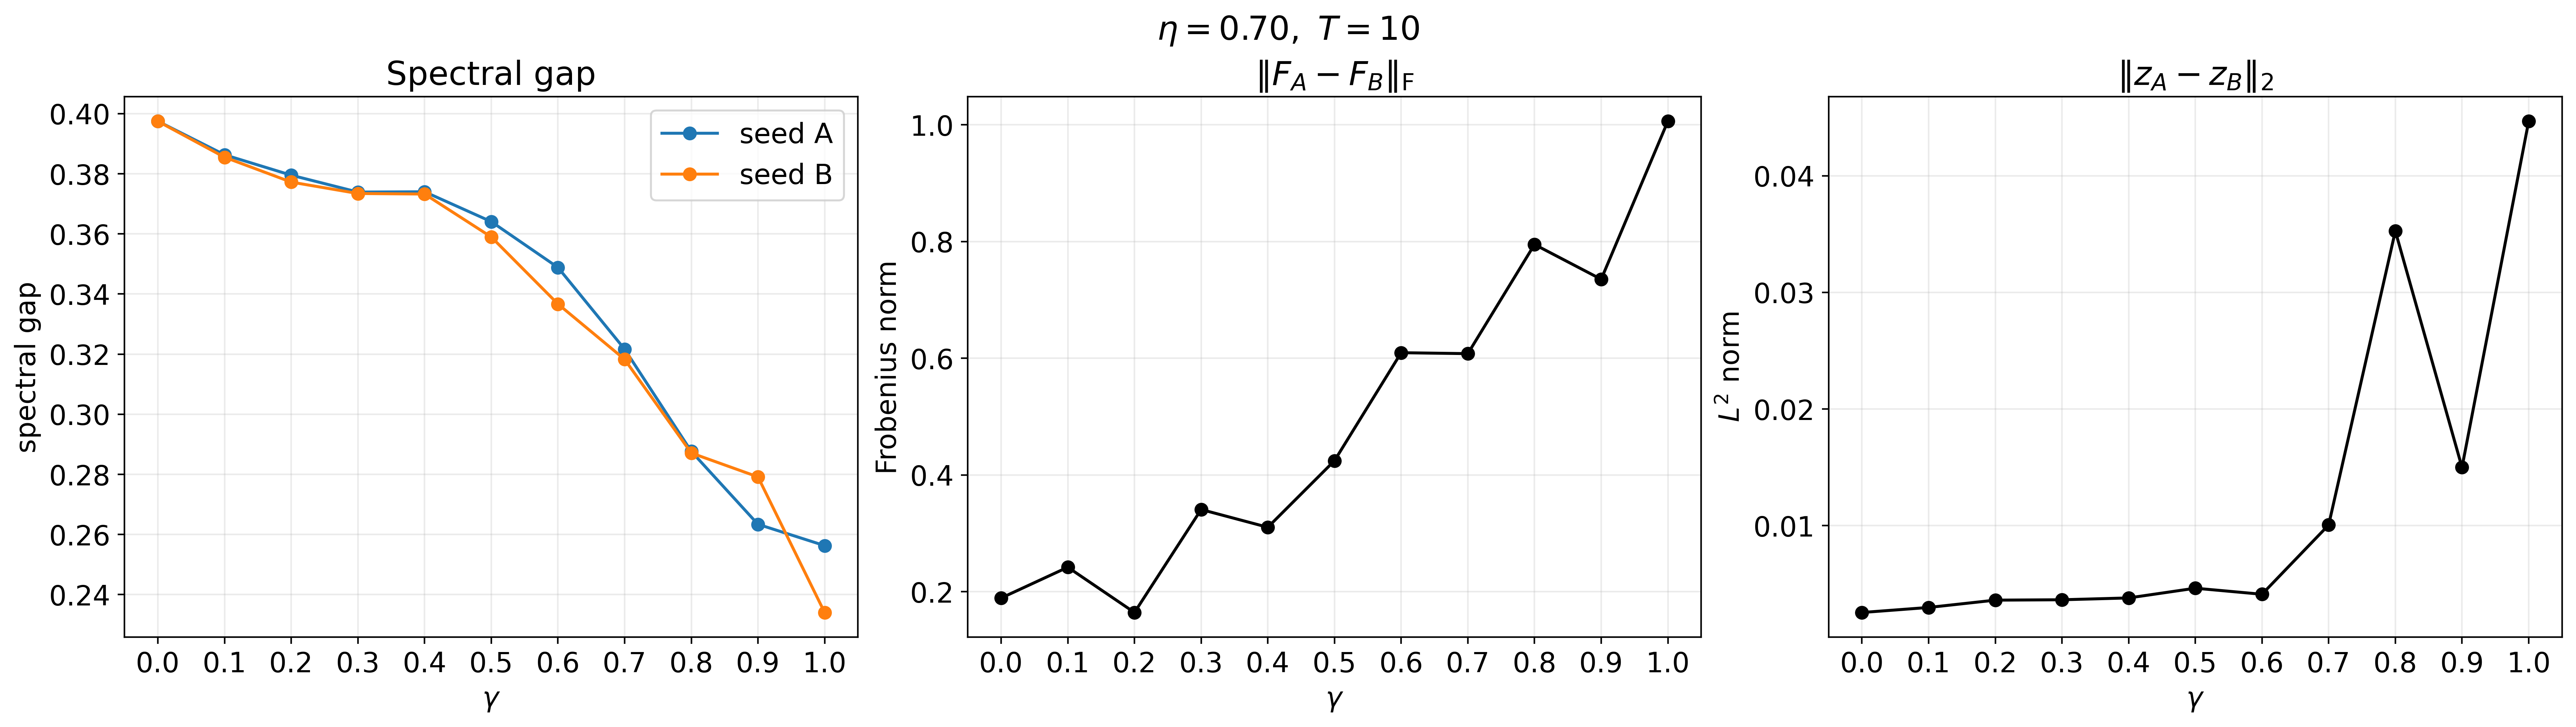
\includegraphics[width=1.0\linewidth]{figures/ct_gamma_eta_0.70_T_10.png}
    \caption{Comparison of two independent runs as $\gamma$ varies, with $\eta=0.70$ and $T=10$. Left: spectral gap of the flux matrix $F$ in \eqref{eq:flux}. Middle: Frobenius norm $\|F_A-F_B\|_F$. Right: $\ell^2$ distance $\|z_A-z_B\|_2$ between the stationary distributions.}
    \label{fig:ct_gamma_eta_0.70_T_10}
\end{figure}
\FloatBarrier

We then examine how the POU temperature and pruning threshold affect this diagnostic.
We select threshold parameters $\eta=0.59,0.63,0.70$, which produce word sets of sizes $188,103,50$, respectively, and compute flux matrices for temperatures $T=0,10,20$.
Together, these choices give nine experimental configurations.
Figure~\ref{fig:ct_gamma_spectral_gap_seed_A_by_temperature} shows the spectral gap of the resulting flux matrices as $\gamma$ varies.
The spectral gap decreases for two related reasons: larger $\gamma$ moves the target distribution away from the $\gamma=0$ distribution used to construct the strata, while larger $T$ concentrates each word on closer plans and therefore reduces its effective support.
\begin{figure}[!htbp]
    \centering
    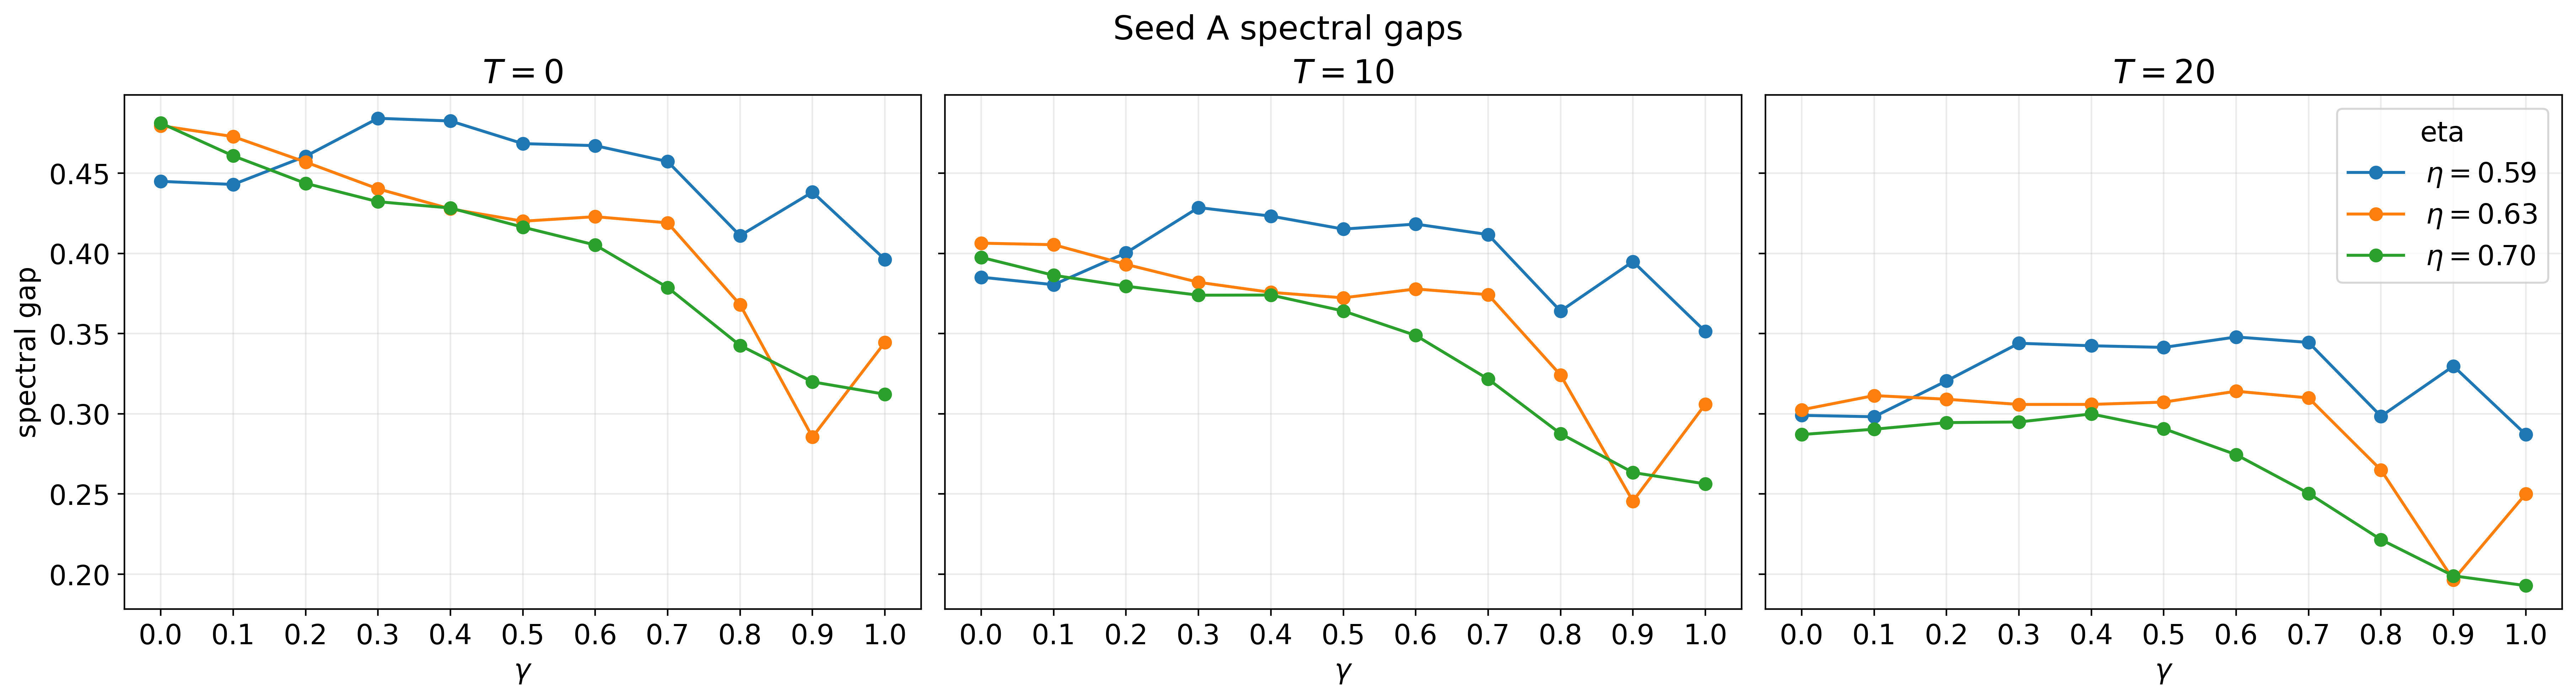
\includegraphics[width=1.0\linewidth]{figures/ct_gamma_spectral_gap_seed_A_by_temperature.png}
    \caption{Spectral gap of the flux matrix $F$ in \eqref{eq:flux} for seed A as $\gamma$ varies. Each panel fixes the temperature $T$ in the POU kernel \eqref{eq:psi_relative}, while colors indicate the threshold parameter $\eta$ used in Algorithm~\ref{alg:eta_greedy_subcover}.}
    \label{fig:ct_gamma_spectral_gap_seed_A_by_temperature}
\end{figure}

% internal comment: we have nc results but it's incomplete so i don't plan to include it
% \subsection{North Carolina}\label{sec:north_carolina}
% We next apply the pipeline to redistricting plans of North Carolina, where $|V|=2671$ precincts are partitioned into $I=14$ congressional districts.
% In the NC case, the elbow appears at a larger $K$ due to the increase in the number of districts.
% We see that the dispersion drops sharply around $K=129$, as shown in Figure~\ref{fig:nc_elbow}.
% \begin{figure}[!htbp]
%     \centering
%     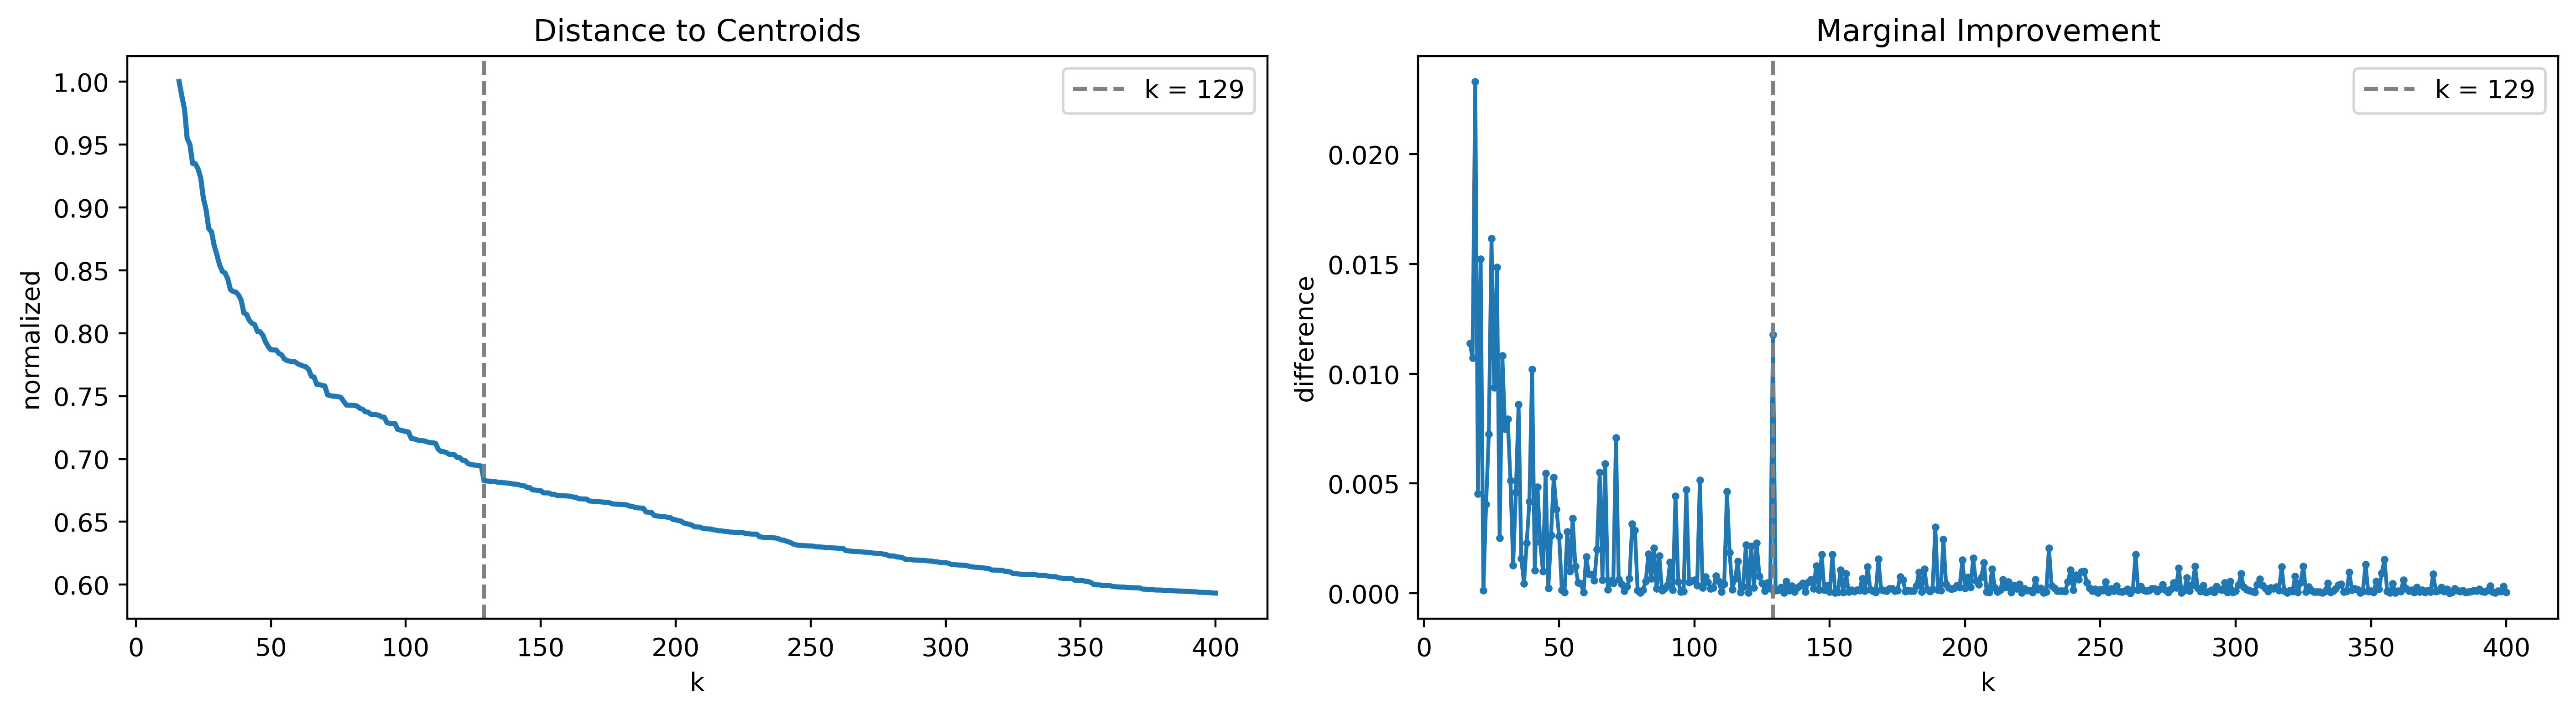
\includegraphics[width=1.0\linewidth]{figures/nc_elbow.png}
%     \caption{Elbow plots for NC - left: dispersion metric against number of clusters, right: marginal improvements on the dispersion metric by taking consecutive differences.}
%     \label{fig:nc_elbow}
% \end{figure}
% Figure~\ref{fig:nc_merge_129} visualizes the \hccultra merges around this elbow, suggesting an optimal alphabet size around $K=129$.
% \begin{figure}[!htbp]
%     \centering
%     \includegraphics[width=1.0\linewidth]{figures/nc_merge_129.png}
%     \caption{The merges of \hccultra around the elbow in the NC case. Each row represents a merge performed by \hccultra of two clusters into one (indicated by left, right and merged). The color on a precinct $p$ indicates the fraction of districts within a cluster that contains $p$.}
%     \label{fig:nc_merge_129}
% \end{figure}

% We set an alphabet size of $K=129$ and choose a big enough beam search width of $L=1000$ to capture all relevant words.
% Figure~\ref{fig:nc_top5_word_before_prune} visualizes the five words with the largest estimated stratum weights before pruning; as in the CT case, several of these high-weight words are near-duplicates that differ only by small local letter substitutions.
% \begin{figure}[!htbp]
%     \centering
%     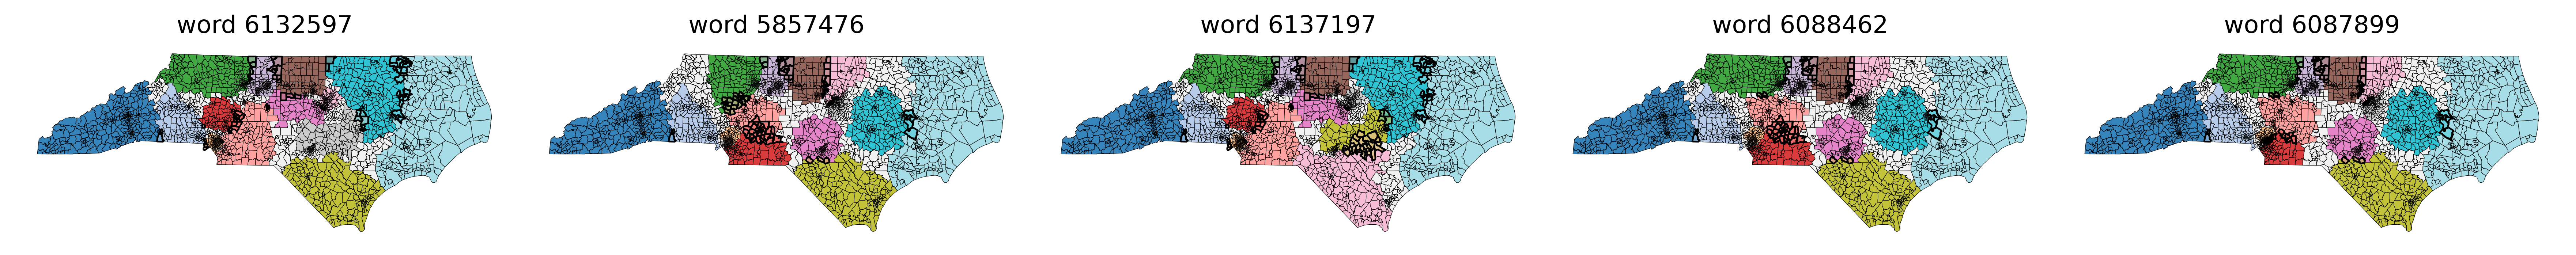
\includegraphics[width=1.0\linewidth]{figures/nc_top5_word_before_prune.png}
%     \caption{Top five words (by number of plans covered) before pruning. We visualize words by plotting the letters with different colors. Intersections between letters are highlighted in black lines.}
%     \label{fig:nc_top5_word_before_prune}
% \end{figure}

% We again construct the pruned set $\mathcal{S}_\eta$ using the two-stage greedy subcover in Algorithm~\ref{alg:eta_greedy_subcover}.
% Figure~\ref{fig:nc_top5_word_after_prune} shows that, after pruning, the top words are more diverse and correspond to distinct plan motifs rather than minor variations.
% Word $6132597$ covers most plans, hence appears in both Figure~\ref{fig:nc_top5_word_before_prune} (by definition) and Figure~\ref{fig:nc_top5_word_after_prune} since it is selected first in the initial greedy subcover of Algorithm~\ref{alg:eta_greedy_subcover}.
% \begin{figure}[!htbp]
%     \centering
%     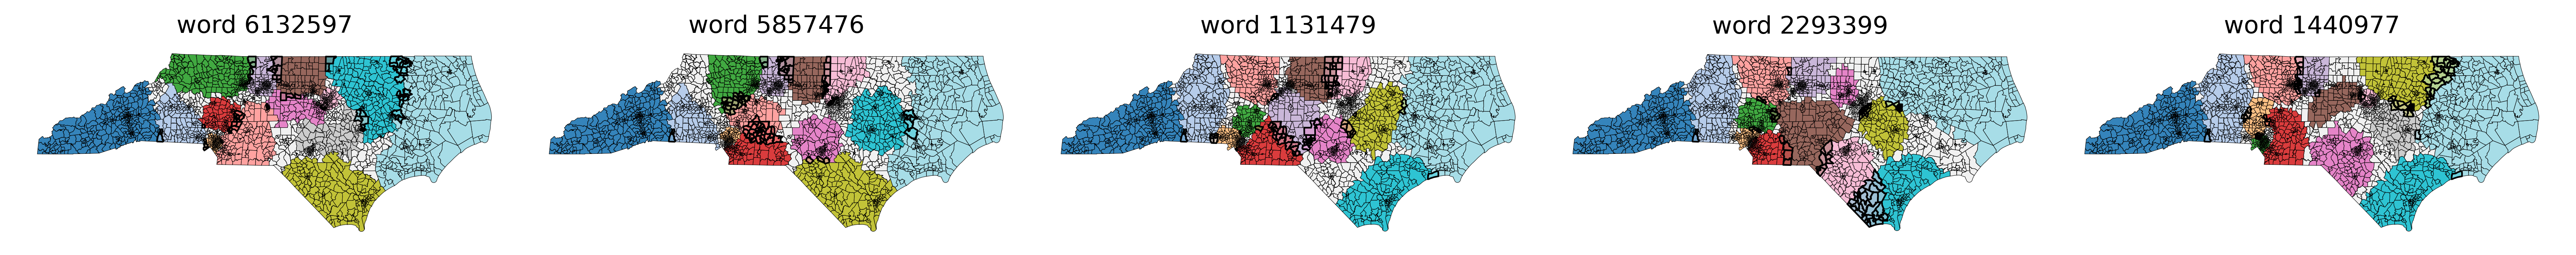
\includegraphics[width=1.0\linewidth]{figures/nc_top5_word_after_prune.png}
%     \caption{Similar to Figure~\ref{fig:nc_top5_word_before_prune} but for the pruned set $\mathcal{S}_\eta$ produced by the two-stage greedy subcover. Pruning removes near-duplicate strata while maintaining coverage of the sampled ensemble, yielding a more compact and interpretable set of representative words.}
%     \label{fig:nc_top5_word_after_prune}
% \end{figure}
% \FloatBarrier
